\documentclass[11pt, a4paper]{article}
\usepackage{amsmath, amssymb}
\usepackage{booktabs}
\usepackage{tabularx}
\usepackage{minted}
\usepackage{tcolorbox}
\usepackage{graphicx}
\usepackage[utf8]{inputenc}
\usepackage[T1]{fontenc}
\usepackage{geometry}
\geometry{margin=1in}

% Custom commands and environments
\newcommand{\sta}{\textbf{\sffamily [CRITICAL / EXAM]\ }}

\newenvironment{important}
  {\begin{tcolorbox}[colback=blue!5!white, colframe=blue!75!black, arc=1mm, boxrule=1pt]}
  {\end{tcolorbox}}


\begin{document}
% Lecture Notes: Multiple Sequence Alignment (Part 2)

% Defining environments and commands as requested since preamble access is restricted


\section{Introduction: Extending Alignments via Weighted Dynamic Programming}

Before discussing how to build alignments from scratch, it is crucial to understand how to add a new sequence to an existing alignment. When we have an alignment of multiple sequences, we can represent it as a profile (a frequency matrix for each column). 

To align a new single sequence to this existing profile, we use a variation of dynamic programming called \textbf{weighted dynamic programming}. Instead of comparing a character from the new sequence against a single character, we compare it against an entire column of the profile.
The score for a specific position is computed by checking the new character against all possible symbols in the profile column (including gaps), weighting the standard match/mismatch/gap penalties by the fractional presence of those symbols in the profile. 
\sta This weighted profile alignment forms the foundational operation for progressively merging larger sets of sequences.

\section{Progressive Multiple Alignments}

The exact computation of a multiple sequence alignment (MSA) using a multidimensional hypercube becomes computationally intractable for more than a few sequences. Therefore, modern bioinformatics relies heavily on heuristic methods. The de facto standard for this is the progressive alignment approach.

\begin{important}
  \textbf{Progressive Alignment}: A heuristic algorithm for multiple sequence alignment that iteratively aligns pairs of sequences (or alignment profiles) by following their evolutionary history backwards. It starts by aligning the most closely related sequences and progressively adds more distant sequences or clusters.
\end{important}

The core rationale behind this approach is error minimization. In MSA, placing a gap in the wrong position permanently degrades the alignment score. Closely related sequences naturally require fewer gaps to align, meaning the algorithm is less likely to make a placement error. Once these highly reliable "core" alignments are built, they serve as robust guides for aligning more distant, error-prone sequences.

\textbf{Example:} Aligning the English word \textit{sugar} and the French \textit{sucre}.
If we align these two words in isolation, it might be ambiguous whether to place gaps to align the "r"s. However, if we first build an alignment of more closely related words (e.g., \textit{zuker} and \textit{zukero} in other languages), that intermediate profile will strongly indicate that the "r" appears consistently at a specific position, successfully guiding the correct alignment of the more distant English and French variations.

To define the order of operations, the algorithm requires a \textbf{guide tree}. 

\begin{center}
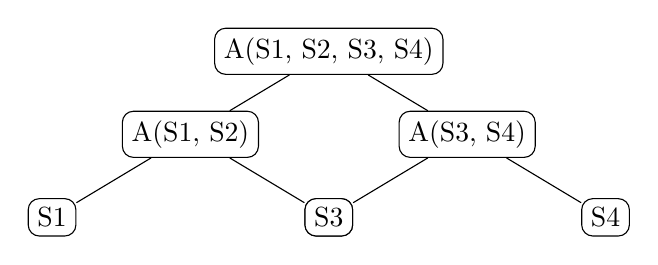
\begin{tikzpicture}[sibling distance=10em, level distance=3em,
  every node/.style = {shape=rectangle, rounded corners, draw, align=center, fill=white}]
  \node {A(S1, S2, S3, S4)}
    child { node {A(S1, S2)}
      child { node {S1} }
      child { node {S2} } }
    child { node {A(S3, S4)}
      child { node {S3} }
      child { node {S4} } };
\end{tikzpicture}
\end{center}

As shown in the tree above, the algorithm never explicitly evaluates the sum-of-pairs (SP) score of the final alignment. Instead, it constructs the solution step-by-step:
\begin{enumerate}
    \item Align S1 with S2 to build the alignment profile A(S1, S2).
    \item Align S3 with S4 to build the alignment profile A(S3, S4).
    \item Align profile A(S1, S2) with profile A(S3, S4) to derive the final multiple alignment.
\end{enumerate}

\section{Building the Guide Tree and Hierarchical Clustering}

A core "chicken and egg" problem arises: to build the MSA, we need an evolutionary guide tree, but to accurately determine evolutionary history, we usually need the MSA. The solution is to estimate the tree on the fly using a greedy strategy based on pairwise similarities. The governing assumption is: \textit{"The more two strings are similar, the more recent is the evolutionary event that produced them."}

This process is fundamentally a form of \textbf{agglomerative hierarchical clustering}. 
Every time we align two strings, we put them in the same cluster. When we align a string to a profile, we add it to an existing cluster. When we align two profiles, we merge two clusters.

\subsection{Algorithm for Tree Construction}
We build the tree moving "back in time" from the leaves (the input sequences) to the root (the final alignment):
\begin{enumerate}
    \item Compare all initial sequences to compute their pairwise alignment distances.
    \item \textbf{Greedy step:} Choose the pair with the minimal distance (e.g., S1 and S2), align them, and build their profile A(S1, S2). This alignment replaces S1 and S2 in the pool of objects.
    \item Recompute distances between the newly formed profile and all remaining objects. (Note: Distances between unchanged objects, like S3 and S4, do not need to be recomputed).
    \item Repeat the greedy step until only two objects remain, then merge them into the final alignment.
\end{enumerate}

\subsection{Measuring Distances in Clustering}
To execute the algorithm, we must define what "distance" means for different combinations of objects:

\begin{itemize}
    \item \textbf{String to String:} The distance derived from their standard pairwise alignment score.
    \item \textbf{String to Cluster (Profile):} How do we define the distance between a single sequence and a profile?
        \begin{itemize}
            \item \textit{Minimum distance:} Distance to the closest string in the cluster.
            \item \textit{Maximum distance:} Distance to the farthest string in the cluster.
            \item \textit{Average distance:} The weighted average of distances to all strings in the cluster (this is the standard choice for sequences).
        \end{itemize}
    \item \textbf{Cluster to Cluster:} Similarly evaluated via minimum, maximum, or average distances of all possible string pairs across the two clusters.
\end{itemize}

\begin{important}
  \textbf{Neighbor Joining}: An advanced clustering methodology and variation of the average distance principle. It defines distance based on the relationship between two objects' closeness to each other versus their closeness to everything else. 
\end{important}

If two objects are close to each other, but also very close to a third cluster, it might be premature to merge them. Conversely, if two objects are moderately distant from each other, but extremely distant from everything else in the dataset, they are strong candidates for merging. Neighbor joining is highly favored in MSA because it generally produces more reliable guide trees.

% [IMAGE: Hierarchical clustering dendrogram of large DNA viruses (e.g., Mamavirus and Mimivirus). The edge length is proportional to the computed distance, visually indicating closeness between items and clusters.]

\section{The Local Multiple Alignment Problem}

Global MSA forces full-length alignment, but often biological significance is restricted to small, conserved sub-regions. We must therefore address the \textbf{Local Multiple Alignment Problem}.

\subsection{Motivation and Use Case}
A typical scenario involves identifying binding sites for transcription factors (e.g., data derived from a ChIP-seq experiment). 
\textbf{Example:} We possess thousands of DNA sequences, each roughly 1,000 nucleotides long. We know a specific protein binds somewhere within each sequence. 
This binding site (motif) is short (usually 5–20 bases) and highly conserved, though it allows for slight mismatches. Critically, these biological motifs generally do \textit{not} contain insertions or deletions (gaps). Our goal is to extract these small substrings to discover the underlying biological pattern.

\subsection{Formalization: Motif Finding}
Because local optimal alignments of this type typically do not feature gaps, the formulation becomes narrower and easier in one sense, but combinatorial in another.

\begin{important}
  \textbf{Motif Finding Problem}: Given a set of $k$ input strings and a fixed substring length $w$, find a set of $k$ substrings (exactly one per input string) that produces the gapless multiple alignment of maximum score according to an evaluation function $f(x)$.
\end{important}

Any candidate solution is simply defined by a vector of integers $(p_1, p_2, \dots, p_k)$ representing the starting index of the substring in each of the $k$ input strings.
Despite ignoring gaps, this is a classic NP-hard combinatorial optimization problem. Assuming each string has length $n$, there are $n-w+1$ possible substrings per string. For $k$ strings, the total search space is $(n-w+1)^k$. 

\section{Scoring Motifs: Information Content}

For local MSA without gaps, we rely on a scoring function borrowed from information theory rather than the standard sum-of-pairs score. 
We represent the gapless alignment as a profile where $f_{i,j}$ is the fractional frequency of symbol $i$ (e.g., A, C, G, T) in column $j$. The frequencies in any column always sum to 1.

\begin{important}
  \textbf{Information Content (IC) Score}:
  \[ IC(P) = \sum_{i=1}^{4} \sum_{j=1}^{w} f_{i,j} \log_{2} \frac{f_{i,j}}{p_i} \]
  where $f_{i,j}$ is the observed frequency of nucleotide $i$ in column $j$, and $p_i$ is the background probability of nucleotide $i$ in the genome.
\end{important}

\sta For standard DNA, the background probability $p_i$ is assumed to be a random uniform $1/4$ (or 25\%). 

\textbf{Justification for the formula:}
\begin{itemize}
    \item \textbf{Minimum Score (Random):} If a column contains random nucleotides, $f_{i,j} = 1/4$. The term becomes $\log_2(1) = 0$. The score is naturally $0$ for noise.
    \item \textbf{Maximum Score (Perfect Conservation):} If a column is 100\% composed of a single nucleotide (e.g., all 'A's), the term becomes $1.0 \times \log_2(1.0 / 0.25) = \log_2(4) = 2$ bits. For a motif of length $w$, the maximum possible score is $2 \times w$.
    \item \textbf{Biological Adjustments:} The background probability can be adjusted based on the organism's GC-content. For example, yeast has a 38\% GC-content, meaning $p_G = p_C = 0.19$, and $p_A = p_T = 0.31$.
\end{itemize}

This measure is equivalent to the \textit{Shannon entropy/uncertainty} from information theory and the \textit{Kullback-Leibler (KL) divergence} from statistics. It allows us to visualize the binding site using a \textbf{Sequence Logo}, where the height of a stack of letters at each position indicates the total Information Content (in bits), and the height of individual letters reflects their relative frequency.

% [IMAGE: Sequence Logo diagram showing stacked DNA letters A, C, G, T across a motif of length w. The y-axis measures Information Content from 0 to 2 bits. Positions with a single dominant letter (e.g., T) reach nearly 2 bits, indicating high conservation.]

\section{Heuristic Optimization Approaches}

Because the motif finding search space $(n-w+1)^k$ is exponentially large, an exhaustive search—which iteratively compares $O(n^2)$ profiles, then $O(n^3)$, all the way to $O(n^k)$—is completely unfeasible.

\subsection{Greedy Algorithms}
A greedy approach massively reduces time complexity by retaining only the best intermediate solutions. 
Instead of evaluating all combinations:
\begin{enumerate}
    \item Align every substring of $S_1$ with every substring of $S_2$. We get $O(n^2)$ profiles.
    \item Sort these profiles by their IC score and \textbf{keep only the best $n$ profiles}.
    \item Align every substring of $S_3$ to these $n$ profiles, yielding $O(n^2)$ new combinations.
    \item Keep the best $n$, and repeat until all sequences are processed.
\end{enumerate}
While incredibly fast, this method may get "stuck" in a local optimum. If the optimal final alignment relied on a pair from $S_1$ and $S_2$ that ranked $(n+1)$ at step 1, the true global optimum is permanently discarded.

\subsection{Exploring the Search Space (Local Search)}
An alternative strategy views every candidate solution as a discrete point in a $k$-dimensional search space. 

\textbf{Example: MAX-CUT Problem (Binary optimization context)}
MAX-CUT is a classic NP-hard problem where nodes in a graph must be partitioned into two subsets to maximize the number of edges crossing between them. The solution is described by $k$ binary variables. A local search starts with a random assignment (0 or 1 for each node). The algorithm sequentially flips one variable (logical NOT). If the flip increases the number of cut edges ($\Delta f > 0$), it accepts the change. This repeats until no single flip improves the score.

\textbf{Applying Local Search to Motif Finding (Hill Climbing):}
Our variables $X_1, X_2 \dots X_k$ are not binary, but rather integers ranging from $1$ to $(n-w+1)$, representing the starting position in each string.
\begin{enumerate}
    \item Start with an initial random alignment profile $P(0)$ (pick one random substring per sequence).
    \item Select one sequence $S_i$ (variable $X_i$).
    \item Remove the current substring $X_i$ from the profile.
    \item \textbf{Define the neighborhood}: Keep the substrings from all other $(k-1)$ sequences fixed. Iterate through all possible starting positions $j$ in $S_i$.
    \item Insert each candidate substring into the profile and calculate the new IC score.
    \item Choose the position $j$ that yields the steepest increase in the IC score, making it the new value for $X_i$.
    \item Repeat for the next variable, ideally cycling through all variables in a random order, until a full cycle yields no improvement.
\end{enumerate}

% [IMAGE: 2D representation of a search space grid showing "hill climbing". Red paths from random starting nodes traverse to the steepest neighboring nodes, eventually stopping at local maxima. A blue path shows the trajectory to the global maximum, demonstrating dependency on the starting point.]

Because deterministic local search stops at the first local maximum it finds, it must be iterated multiple times from different random starting positions to increase the probability of discovering the global maximum.

\section{Stochastic Search and Optimization}

To mitigate the major flaw of deterministic hill climbing—getting stuck in sub-optimal local maxima—we use stochastic optimization. The fundamental idea is to occasionally accept a "bad" move (a step that decreases the IC score) to escape a local peak and explore new areas of the search space.

\subsection{Simulated Annealing}
In simulated annealing, if a move improves the score ($\Delta f > 0$), it is always accepted. If it worsens the score ($\Delta f \leq 0$), it is accepted with a specific probability:
\[ P[\text{update } X_i] = e^{\frac{\Delta f}{T}} \]
The parameter $T$ represents "temperature". 
\begin{itemize}
    \item At high temperatures (early in the algorithm), the exponent is small, and the probability of accepting a bad move is relatively high, allowing wide exploration.
    \item Over time, $T$ is artificially lowered ("cooled"). As $T \to 0$, the algorithm gradually reverts to a standard, deterministic local search.
\end{itemize}

\subsection{Gibbs Sampling}
Gibbs Sampling is a specific stochastic strategy tailored for the Local MSA problem. Unlike local search (which always picks the absolute best new substring) or simulated annealing (which evaluates a single specific delta), Gibbs sampling evaluates \textit{all} possible substrings for $X_i$ and picks one purely based on a weighted probability distribution.

\begin{minted}{python}
# [pseudocode]
def gibbs_sampling(sequences, motif_length, iterations):
    # 1. Start with random substring positions
    positions = [random_start(seq, motif_length) for seq in sequences]
    
    for _ in range(iterations):
        # 2. Pick a random string variable to update
        i = random_index(sequences)
        
        # 3. Evaluate all possible starting positions in string i
        scores = []
        for p in possible_positions(sequences[i], motif_length):
            profile = build_profile(sequences, positions, exclude=i, new_pos=p)
            scores.append(information_content(profile))
        
        # 4. Calculate total score over all possibilities
        total_score = sum(scores)
        
        # 5. Determine probabilities and pick a new position randomly
        probabilities = [s / total_score for s in scores]
        positions[i] = sample_based_on_probability(probabilities)
        
    return positions
\end{minted}

\textbf{Explanation of the Code:}
This algorithm iteratively refines a motif alignment by treating the starting positions as random variables. It removes one sequence from the current alignment, tests every possible motif position within that sequence against the remaining profile, and computes the Information Content for each. Rather than greedily selecting the position with the maximum score, it normalizes these scores into a probability distribution. The new position is drawn randomly from this distribution. This allows the algorithm to occasionally pick sub-optimal positions, effectively preventing it from getting trapped in local maxima.

\textbf{Walkthrough of the algorithm:}
\begin{enumerate}
    \item Compute $IC(p_j)$ for every possible starting position $p_j$ in the selected sequence $S_i$.
    \item Calculate the total sum of all possible IC scores for the sequence: $IC(S_i) = \sum_{j=1}^{n-w+1} IC(p_j)$.
    \item Accept a new position $p_j$ for variable $X_i$ via a random choice governed by the probability:
    \[ Pr[X_i = p_j] = \frac{IC(p_j)}{IC(S_i)} \]
\end{enumerate}
Because the algorithm's probabilities are not dynamically flattened (unlike the cooling phase of simulated annealing), it remains stochastic indefinitely. Consequently, it is typically run for a fixed number of iterations, and the algorithm reports the best overall solution encountered during the entire run.


\subsection{Summary of the Motif Finding Search Strategy}
To solidify the understanding of these local alignment algorithms, it is helpful to conceptualize the search space directly and summarize the pipeline. 

\textbf{The Grid Analogy vs. String Algorithms:}
\begin{itemize}
    \item In a simple 2D mathematical grid, the "neighborhood" of a candidate solution consists of the directly adjacent nodes (e.g., changing coordinates by $\pm 1$).
    \item In the string-based Motif Finding problem, the neighborhood is vastly larger. For a given dimension (representing one sequence $S_i$), the "neighborhood" encompasses \textit{all} $(n - w + 1)$ possible substring starting points in that sequence, while keeping the starting points in all other $(k - 1)$ sequences strictly fixed. 
\end{itemize}

\textbf{Step-by-Step Pipeline Recap:}
\begin{enumerate}
    \item \textbf{Initialization}: We begin with a large dataset (e.g., $1,000$ input strings derived from a ChIP-seq experiment). We select an initial candidate solution by picking one substring of length $w$ from each string. This can be done purely at random or using a heuristic guide.
    \item \textbf{Fixing and Exploring}: We pick the first variable (representing the starting position in the first string) and keep the remaining $999$ variables fixed. 
    \item \textbf{Evaluating the Neighborhood}: We slide a window of size $w$ across the entire length of the first string. For every possible position, we temporarily build the profile with the $999$ fixed strings and evaluate the Information Content (IC) score.
    \item \textbf{Updating}: 
    \begin{itemize}
        \item In a \textit{deterministic local search} (Hill Climbing), we permanently adopt the position that yields the absolute highest IC score in that neighborhood.
        \item In a \textit{stochastic search} (Simulated Annealing or Gibbs Sampling), we evaluate all options and may select a suboptimal position based on a weighted probability distribution. This intentionally allows for a temporary decrease in the overall IC score to escape local maxima.
    \end{itemize}
    \item \textbf{Iteration}: We move to the second string, keep the (newly updated) first string and the remaining $998$ strings fixed, and repeat the evaluation process. We cycle through all variables—ideally in a randomized order—until the algorithm converges or reaches a predefined iteration limit.
\end{enumerate}

\sta While deterministic searches must be run numerous times from different random starting points to combat the issue of local maxima, stochastic methods inherently model this escape probability, making them significantly more robust for the highly complex search spaces typical of biological sequences.

% [IMAGE: Summary diagram of the Motif Finding process showing a set of unaligned sequences on the left, the iterative sliding window search process in the middle, and the final extracted binding motif aligned to create a Sequence Logo on the right.]

\section{Historical Context and References}

The mathematical and algorithmic foundations discussed for Multiple Sequence Alignment draw upon decades of cross-disciplinary research:

\begin{itemize}
    \item \textbf{Information Theory}: The Information Content (IC) score used to evaluate gapless local alignments is derived directly from the Shannon Entropy formula introduced by Claude E. Shannon in 1948 (\textit{A Mathematical Theory of Communication}).
    \item \textbf{Statistics}: The scoring mechanism is mathematically equivalent to the Kullback-Leibler (KL) Divergence (1951), which measures how one probability distribution diverges from a second, expected reference distribution (in our case, the background nucleotide frequencies).
    \item \textbf{Data Mining}: The progressive multiple alignment methodology is fundamentally an application of Agglomerative Hierarchical Clustering. The visual representation of these clusters via dendrograms (guide trees) is heavily used in comparative genomics (e.g., Bajrai L.H. et al., 2016, regarding the clustering of large DNA viruses).
\end{itemize}

\section{Conclusion: The Reality of Biological Computing}

Whether dealing with Global or Local Multiple Sequence Alignment, modern bioinformatics relies almost exclusively on heuristic algorithms due to the NP-hard nature of finding exact solutions. 

\begin{important}
  \textbf{Core Takeaway}: Perfectly optimal mathematical solutions are computationally inaccessible for realistically sized biological datasets. However, well-designed heuristics—especially those guided by evolutionary logic (Progressive Alignment) or statistical sampling (Gibbs Sampling)—consistently yield highly accurate, biologically meaningful results.
\end{important}

\end{document}